\documentclass{article}
\usepackage{tikz}
\usetikzlibrary{intersections}

\begin{document}

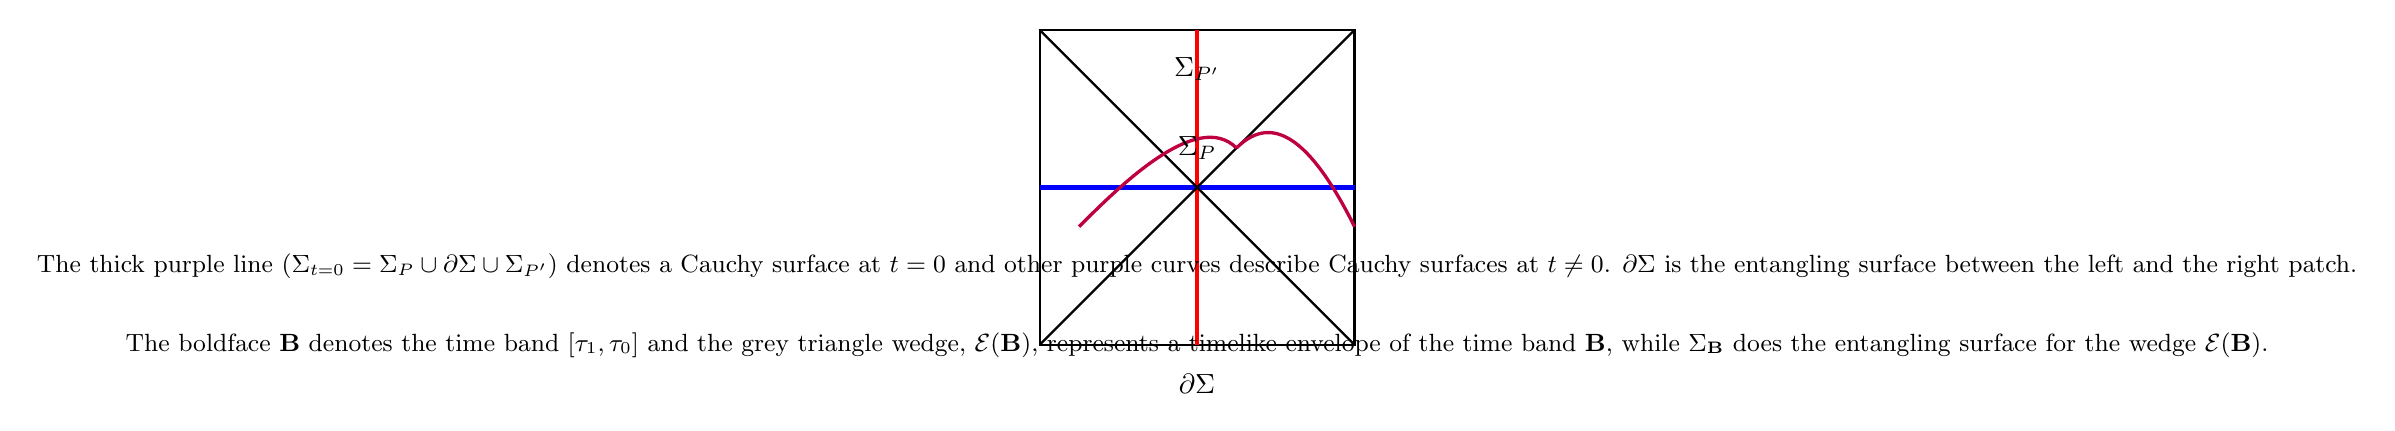
\begin{tikzpicture}[scale=1]
    % Draw the boundary lines of the square
    \draw[thick] (0,0) -- (4,0) -- (4,4) -- (0,4) -- cycle;
    \draw[ultra thick, blue] (0,2) -- ++(4,0);
    \draw[ultra thick, red] (2,0) -- ++(0,4);
    
    % Draw the diagonal lines
    \draw[thick] (0,4) -- (4,0);
    \draw[thick] (4,4) -- (0,0);
    
    % Draw the Cauchy surfaces
    \draw[very thick, purple] (0.5,1.5) .. controls (1,2) and (2,3) .. (2.5,2.5);
    \draw[very thick, purple] (2.5,2.5) .. controls (3,3) and (3.5,2.5) .. (4,1.5);
    
    % Label the Cauchy surfaces and the entangling surface
    \node at (2,-0.5) {$\partial \Sigma$};
    \node at (2,2.5) {$\Sigma_P$};
    \node at (2,3.5) {$\Sigma_{P'}$};
    
    % Describe the Cauchy surfaces
    \node at (2,1) {\small The thick purple line ($\Sigma_{t=0} = \Sigma_P \cup \partial \Sigma \cup \Sigma_{P'}$) denotes a Cauchy surface at $t=0$ and other purple curves describe Cauchy surfaces at $t \neq 0$. $\partial \Sigma$ is the entangling surface between the left and the right patch.};
    
    % Additional description
    \node at (2,0) {\small The boldface ${\bf B}$ denotes the time band $[\tau_1, \tau_0]$ and the grey triangle wedge, ${\cal E}(\bf B)$, represents a timelike envelope of the time band ${\bf B}$, while $\Sigma_{\bf B}$ does the entangling surface for the wedge ${\cal E}(\bf B)$.};
\end{tikzpicture}

\end{document}